\documentclass[tikz, border=10pt]{standalone}
\usetikzlibrary{datavisualization, datavisualization.formats.functions}

\def\pOne{200}
\def\endYear{25}
\def\pTwo{150}
\def\inflation{5}

\begin{document}
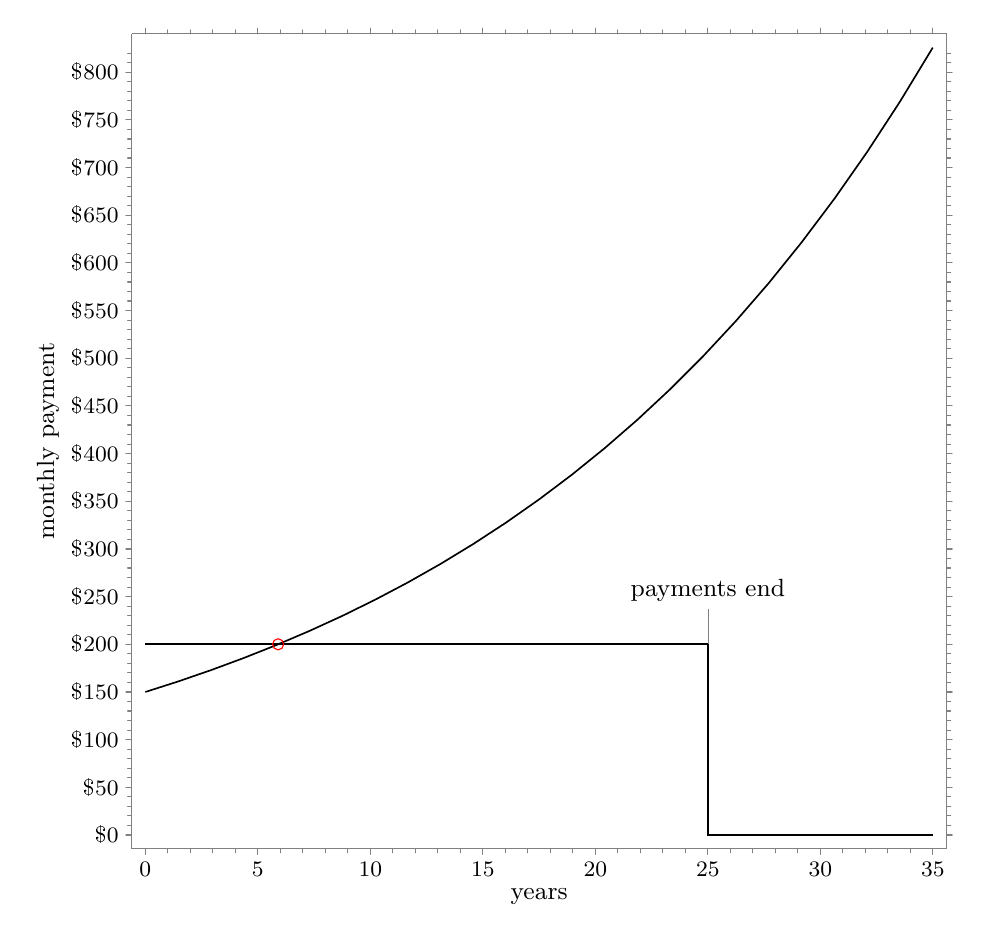
\begin{tikzpicture}[baseline]
  \datavisualization [
    scientific axes,
    visualize as line/.list={payment1, payment2},
    payment1={
        pin in data={text={payments end}, when=x is \endYear},
    },
    all axes={padding=.5em},
    x axis={
        label={years},
        length=10cm,
        ticks={
            step=5, 
            minor steps between steps=4}
        },
    y axis={
        label={monthly payment},
        attribute=y,
        scaling=min at 0cm,
        length=10cm,
        ticks={
            tick prefix=\$, 
            step=50, 
            minor steps between steps=4}
        },
    ]
    data [set=payment1] {
      x, y
      0, \pOne
      \endYear, \pOne
      \endYear, 0
      35, 0
    } 
    data [format=function, set=payment2] {
      var x : interval [0:35]; 
      func y = \pTwo*(1+(\inflation/100))^\value x);
    }
    info{
        \pgfmathsetmacro{\ix}{ln(\pOne/\pTwo)/ln((1+(\inflation/100)))} 
        \draw[red] (visualization cs: x={\ix}, y={\pOne}) circle[radius=2pt];
    };
\end{tikzpicture}
\end{document}